\par Le membre du groupe responsable de cette partie était Antoine Vallée.

\par Notre jeu étant un Shoot Them All, il nous semblé logique que nous aurions besoin d'un éditeur de niveau. Ce dernier permettrait aux joueurs de renouveler eux même le contenu.
\par Le développeur de l'éditeur a débuté pour la soutenance 3, le début fut laborieux: La prise en main des Winforms, le design de l'éditeur\ldots Mais une fois le tout bien lancé, le développement était bien parti. Toutefois, développer l'éditeur de niveau a été une rude tâche. Il fallait par exemple pouvoir rendre possible l'édition d'un vaisseau déjà placé.
\par Le premier problème se trouvait là, il fallait pouvoir développer un système permettant de se déplacer très aisément dans un fichier de niveau, ce ne fut pas simple, mais d'autres épreuves firent leurs apparitions. Tout d'abord, gérer le temps. En effet, il est impossible d'afficher un niveau entier dans l'éditeur, nous avons donc fractionné ces niveaux en « pages » de 3200ms, puis en colonnes de 400ms. Toutefois, si nous voulions rendre possible l'édition de page précédemment remplies, il fallait pouvoir lire un fichier de niveau et l'interpréter convenablement.
\par La plus grosse difficulté de l'éditeur fut ici: L'interprétation d'un fichier de niveau. Replacer au bon endroit les vaisseaux, dans la bonne colonne, avec l'image correspondante. Cela n'était pas encore possible à la soutenance 3, mais ça l'est pour la version finale.
\par L'interprétation nous permet aussi donc d'importer des fichiers de niveaux: Chaque joueur pourra donc modifier n'importe quel niveau du jeu, qu'il a créé, ou qu'un ami lui a donné. L'éditeur lui permet de tout modifier. L'exportation du niveau du joueur était aussi bien sûr nécessaire, dans le but de sauvegarder ce dernier, et de jouer sur le niveau.
\par Ainsi, l'éditeur est donc très complet: Il regroupe tout le contenu du jeu, il est possible d'importer, d'exporter des niveaux, et donc de les partager avec vos amis ! Même si graphiquement il semble basique, notre éditeur est donc un outils très puissant, qui nous fut d'ailleurs très utile pour construire nos niveaux dans le mode Campagne.
\par Vous pouvez voir ici l'évolution de cet éditeur :

\begin{center}
	\par Soutenance 3:
	\par 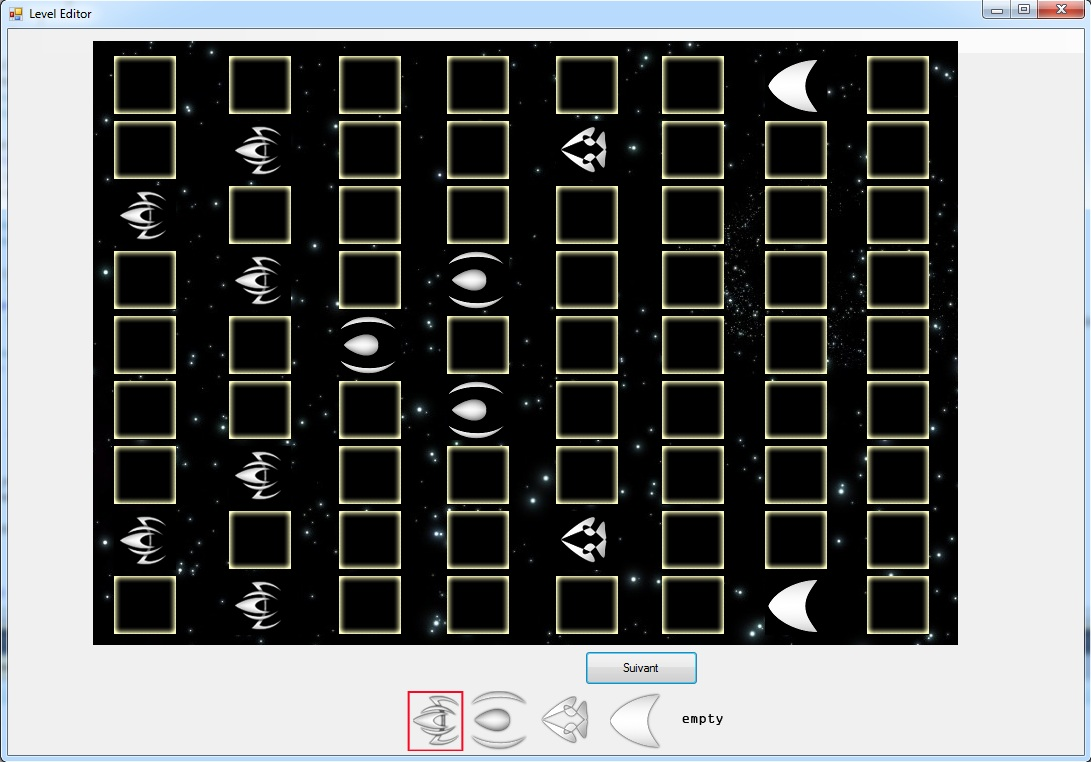
\includegraphics[width=13cm]{images/leveleditor2.jpg}
	\vspace{1cm}
	\par Version finale:
	\par 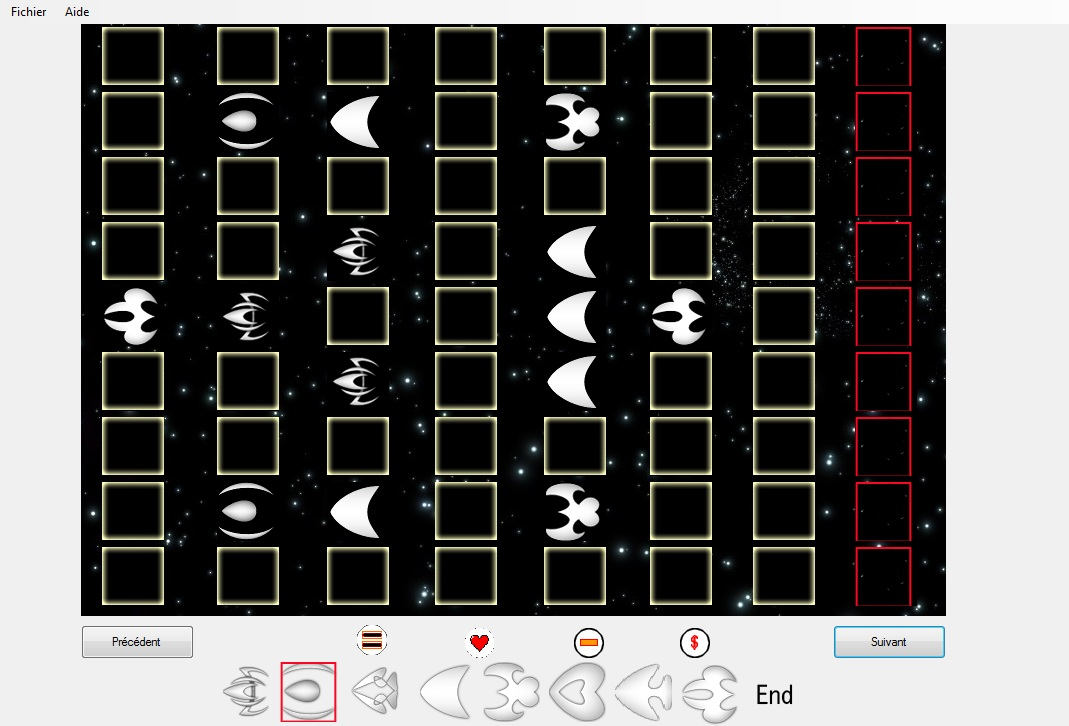
\includegraphics[width=13cm]{images/leveleditor.jpg}
\end{center}